
\chapter{QUADRO METODOLÓGICO}
\par O quadro metodológico é a descrição dos passos realizados para a 
execução do projeto. Serão listados, nos tópicos a seguir, os itens essenciais
no desenvolvimento do trabalho, sendo eles as técnicas, procedimentos, práticas e instrumentos
utilizados, o contexto de aplicação, os participantes, o orçamento, o cronograma
e o tipo de pesquisa utilizado.

\section{Tipo de pesquisa}

\par Para \citeonline[p.42]{pesquisa_social_gil}, a pesquisa tem um caráter
pragmático, é um “processo formal e sistemático de desenvolvimento do método científico. 
O objetivo fundamental da pesquisa é descobrir respostas para problemas mediante
o emprego de procedimentos científicos”.
\par Este projeto terá como base a metodologia de pesquisa aplicada, pois
será desenvolvida uma aplicação inteligente utilizando Algoritmos Genéticos para
o auxílio na tomada de decisão sobre a produção de calças de uma confecção.

\par \citeonline[p.35]{livro_metodos_de_pesquisa} afirmam que o método de
pesquisa aplicada, "objetiva gerar conhecimentos para aplicação prática, dirigidos a
solução de problemas específicos. Envolve verdades e interesses locais."  

\par Segundo \citeonline{livro_metodologia_de_estudo_de_pesquisa}, a pesquisa
aplicada tem como motivação básica a solução de problemas
concretos, práticos e operacionais e também pode ser chamada de pesquisa
empírica pois o pesquisador precisa ir a campo, conversar com pessoas e
presenciar relações sociais.

\section{Contexto de pesquisa}



\par Sabe-se que com a alta competitividade no mercado, empresas cada vez mais
buscam diferenciais competitivos para seus produtos e, neste cenário, a ideia
de redução de custos se torna essencial uma vez que tal redução pode ser
refletida no preço dos produtos permitindo que estes se diferenciem. Dentre
os fatores que viabilizam tais reduções está a otimização de processos que
consistem em organizar os procedimentos relacionados à produção de forma que
estes se tornem mais eficazes.

\par O software desenvolvido neste trabalho visa organizar uma linha de produção
de forma que esta se torne o mais eficiente possível. Será utilizada como
base uma determinada fábrica de confecção de calças situada na cidade de
Cachoeira de Minas - MG, porém a base de conhecimento pode ser aplicada a outros
tipos de negócios que seguem o mesmo padrão de desenvolvimento de produtos.

\par Como já explanado no quadro teórico, a estrutura do algoritmo genético é composta
por populações que são formadas por indivíduos que por sua vez são formados por cromossomos.
Cada indivíduo representa uma solução e cada cromossomo do indivíduo representa uma de suas características. 
Assim ocorre então um processo de cruzamento e mutação a fim de que possam ser gerados novos 
indivíduos que representem soluções ainda melhores que seus antecessores.
As sessões abaixo descrevem como cada um destes elementos foram desenvolvidos no contexto do problema da fábrica de calças.

\par Como cada funcionário da fábrica citada trabalha em sua casa é preciso ter
uma boa forma de distribuir a produção, para que o transporte da materia-prima
seja eficaz contrbuindo para a empresa uma redução de custos e um tempo de
produção melhor.
Para isso, é nescessário que o software conheça os procedimentos de
produção da fabrica, como seus funcionários trabalham e se estão sendo alocados
de forma correta. A aplicação cruza todas essas informações gerando para o
usuario uma relação de como ele deve distribuir a matéria-prima para produção
das peças.

\par Como cada funcionário trabalha em sua casa é preciso saber qual a
melhor rota para se entregar a materia-prima ou recolher o que foi produzido
para que seja passado para a próxima etapa da produção. O software avalia a
melhor rota levando em consideração as peças que precisam ser produzidas, as
habilidades de cada funcionário e se os mesmos não estão alocados em outros
processos de produção. Analisando esses fatos os software sabe a melhor forma
para distribuição da produção e os funcionários tem
suas tarefas distribuidas de forma correta para que não fiquem super alocados ou
sem serviço.


\subsection{Realização da Modelagem da base de dados}

\par O software desenvolvido trabalha com a manipulação de dados cadastrados
para gerar informações que serão utilizadas no processo  de otimização de
produção da fábrica sendo eles muito importantes para que se possa atingir o
objetivo da aplicação. 

\par O banco de dados armazena os dados dos costureiros e suas habilidades,
esses dados são importantes para que cada costureiro seja alocado de forma
correta nas atividades necessárias para produção das calças. Desta forma, se
sabe qual funcionário fabrica a parte da frente da calça, a parte de traz, o
funcionário que coloca o zíper, que faz os bolsos, que junta as partes da peça,
que faz a pintura e entre outras atividades necessárias.

\par A tabela processo tem como finalidade armazenar o modelo peça. Cada
modelo pode possuir atividades diferentes para sua produção, com o cadastro
do modelo da calça é possível separar as atividades de fabricação de cada
modelo, ou seja, um modelo pode conter partes que outros modelos não possuem,
cada modelo é representado por um processo.

\par No banco de dados também possui uma tabela chamada atividade onde são
armazenados os processos e as habilidades dos costureiros necessários para
produção de cada processo.
Como há uma grande variedade de modelos e cortes das peças, os procedimentos
para fabricação podem variar, alguns modelos podem ter procedimentos que em outros
modelos não são necessários.

\par No processo de fabricação tem-se a necessidade de fabricar uma
determinada parte da peça para que outra venha a ser fabricada até que se chegue
no produto final que é a calça. A tabela atividade-ordem é responsável por
organizar as atividades para que sejam executadas na ordem correta. Ela
armazena as atividades 

\par A figura Figura 4 ilustra o que foi descrito acima.

\begin{figure}[h!]
	\centerline{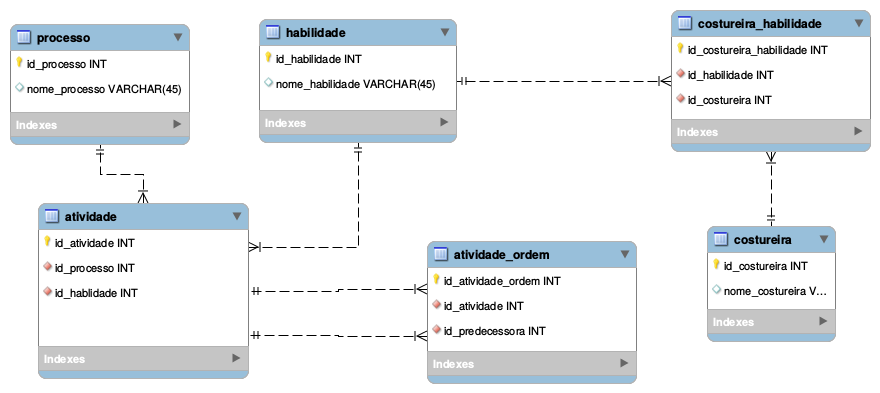
\includegraphics[scale=0.6]{./imagens/model_tcc.png}}
	\caption[Modelo do banco de dados]
	{Modelo do banco de dados \textbf{Fonte:} Desenvolvido pelos autores}
	\label{fig:exemplo1}
\end{figure}

\subsection{Framework de desenvolvimento}
\par Primeiramente é necessário ressaltar que, para o desenvolvimento da aplicação, foi utilizada uma base desenvolvida pelo professor Artur Barbosa durante as aulas de sistemas especialistas, do VII período do curso de sistemas de informação nesta universidade.
Esta base também denominada \textit{framework}, define regras a serem seguidas no desenvolvimento de cada elemento
de um algorítimo genético. Este \textit{framework} é definido dentro da seguinte estrutura:

 \begin{itemize}
 	
 	\item Classe \texttt{GAModel}:
 		\par A classe \texttt{GAModel} é basicamente a classe mãe de todos os elementos de um algoritmo genético, ela representa o modelo que irá armazenar a população de indivíduos além de ser a classe que armazena os parâmetros que definem as configurações do algoritmo, tais como, tipo de cruzamento, tipo de mutação, tamanho da população etc.
 		
 		\par A classe contém os seguintes atributos:
 		
 		\begin{itemize} 
 			\item \textit{populationSize}:
	 			Este atributo define qual será o tamanho da população, ou seja, quantos indivíduos irão formar cada população;
	 			
	 		\item \textit{generationQuantity}:
		 		Como já explicado anteriormente, o processo de cruzamento e mutação se repete até que o número de indivíduos, definido 
		 		no atributo anterior, seja atingido formando assim uma nova população e então, por sua vez, este processo de geração 
		 		de novas populações se repete até que seja atingido um número de gerações definido pelo programador. Este atributo 
		 		representa esta quantidade;
		 		
		 	\item{elitism}:
			 	Atributo do tipo \textit{boolean} que representa se o algoritmo vai ter a função de elitismo. Esta função, como já foi
			 	explicado anteriormente, quando está ativada (com valor \textit{true}), no momento de começar a se criar uma nova população os dois melhores indivíduos da população que será substituída já começam a fazer parte da nova população, antes de começar o processo de cruzamento e mutação. Este mecanismo garante que a nova população terá pelo dois indivíduos iguais ao da antiga população, o que irá impedir que a nova população seja pior que a primeira;
			 	
			 \item{foreignIndividualRate}:
				 
				 
			 \item{mutationRate}:
				 Como descrito no quadro teórico, a mutação é o fato de realizar pequenas alterações no indivíduo a fim de que este possa se tornar ainda melhor. Este parâmetro define uma porcentagem, geralmente baixa, que define quando o indivíduo sofrerá mutação ou não. Esta questão ficará mais claras mais abaixo, quando será explicado o passo a passo da execução do algoritmo.
				 
			  \item{mutationQuantity}:
				  Caso a mutação for ocorrer para o indivíduo, a alteração aleatória será feita nos cromossomos. Este parâmetro define quantos cromossomos do indivíduo deve ser alterado pela mutação;
				  
			  \item{selectionType}:
				  Conforme descrito no quadro teórico, existem várias formas de seleção dos indivíduos para realizarem o cruzamento. Este parâmetro define qual será a forma escolhida pelo programador ao implementar o seu problema. No \textit{framework} este parâmetro é do tipo \texttt{enum} e pode assumir 2 valores o \textit{ROULETTE}, que representa o método roleta e o \textit{CLASSIFICATION}, que representa o método de classificação;
				  
			 \item{crossType}:
				 Assim como a seleção, existe diversas formas de fazer o cruzamento dos indivíduos. Este atributo, também do tipo \texttt{enum} representa a forma de cruzamento e pode receber os valores \textit{Binary}, \textit{Permutation}, \textit{Uniform} e \textit{Aritmetic};
				 
			 \item{mutationType}:
				 Segue as mesma forma que o selectionType e o crossType e pode assumir os valores \textit{Permutation}, \textit{Binary} e \textit{Numerical}.
 			
 		\end{itemize}
 	
 	\item Classe \texttt{Individual}:
	 	\par A classe abstrata \texttt{Individual}, encontra-se dentro do pacote edu.univas.edu.tcc.gacore e  
	 	representa a estrutura básica de um indivíduo. A classe contém uma \texttt{lista} do tipo \texttt{Cromossomo}, que será 
	 	descrito mais abaixo, que contém uma coleção de objetos que representam as características da solução. 
	 	\par A Classe contém ainda um atributo chamado \texttt{valor} que irá armazenar a qualidade, ou seja, qual é o custo
	 	da solução representada pelo indivíduo, tal valor é recebido no retorno da operação calcularValor() descrita abaixo.
	 	\par Com relação as operações, além dos \textit{getters and setters} e o construtor, que recebe a lista de cromossomos como
	 	parâmetro, a classe contém a operação abstrata \texttt{calcularValor()}, esta operação é quem realiza a função de avaliação, 
	 	explicada anteriormente, que mede a qualidade do indivíduo. Desta forma, ao utilizar este \textit{framework}, a
	 	classe que representa o indivíduo do problema deve herdar desta classe  \texttt{Individual}. Fazendo isso tal classe passará a ter uma
	 	lista de cromossomos e o atributo que representa o seu valor e a classe obrigatoriamente terá que implementar a operação 
	 	\texttt{calcularValor()}, já que esta é abstrata na classe mãe, permitindo assim que o programador desenvolva a função de avaliação específica para o seu problema.
 
	\item Classe \texttt{Chromosome}:
		\par 
 	
 	\item Classe \texttt{IndividualPair}:
		 \par
 	
 	
 	\item Classe \texttt{GAController}:
 	
 	
 \end{itemize}

 A Figura X representa o diagrama de classes que demonstra a estrutura em questão.
 (Desenhar diagrama de classe do framework no ASTAH)


\par Posterior a definição das regras de desenvolvimento, os próximos tópicos apresentam a implementação 
dos elementos, seguindo as definições do \textit{framework}.


\subsection{Definição do indivíduo e Cromossomos}
\par O processo de definição indivíduo foi o primeiro passo do desenvolvimento da aplicação. Isso 
se deu devido ao fato de que o indivíduo é a parte crucial para que se possa definir a lógica a ser seguida para
a definição da população inicial, o tipo de cruzamento a função de avaliação etc.
 

\par Em um primeiro momento, o modelamento do indivíduo e seus cromossomos foi feito da seguinte forma:
Foi criado uma classe Java para representar o individuo denominada ProcessoIndividuo, esta classe é filha 
da classe Individual definida no framework.




todavia verificou-se que o algoritmo poderia apresentar problemas de performance. Um outro fator que 
influenciou para que se pensasse em uma nova abordagem foi o fato de somente parte da inteligência da distribuição
das horas ficarem sob responsabilidade do algoritmo, assim, sob a orientação do professor Artur Barbosa (mudar nome), 
o indivíduo e seus cromossomos foram desenvolvidos como descrito abaixo. Esta nova forma também facilitou o processo 
de cruzamento e mutação que será explanado mais adiante.


\section{Instrumentos}

\par Segundo \citeonline{aula_joelma_26_03_15}, instrumentos de pesquisa são a
forma que os dados serão coletados para a realização do trabalho, podendo ser,
dentre outras formas, por meio de reuniões, questionários e entrevistas. Para
este projeto utilizaremos os instrumentos descritos nas subsessões a seguir.

\subsection{Entrevistas}
\par Segundo \citeonline{metodoliga_qualitativas_na_sociologia}, entrevista é
uma interação entre duas pessoas em que uma representa o entrevistador, 
que através de perguntas, obtêm informações por parte de outra pessoa que
representa o entrevistado.


% entrevista é um
% “processo de interação social entre duas pessoas na qual uma delas, o entrevistador,
% tem por objetivo a obtenção de informações por parte do outro, o entrevistado”



\par Será realizada uma entrevista com o dono da empresa de confecção com o
objetivo de entender seu modelo de negócio para que então seja possível começar
a fazer o levantamento dos requisitos do sistema. Para
\citeonline[p.128]{pressman2011engenharia}, levantamento de requisitos de
software consiste em

\begin{citacao}
perguntar ao cliente, aos usuários e aos demais interessados quais são os
objetivos para o sistema ou produto, o que deve ser alcançado, como o sistema ou
produto atenda às necessidades da empresa e, por fim, como o sistema ou produto
deve ser utilizado no dia a dia.
\end{citacao} 


\subsection{Reuniões}
\par De acordo com \citeonline{ref_reuniao}, reunião é o ajuntamento de
pessoas para se tratar de um determinado assunto em que é necessário que se
tenha conclusões sobre as questões que foram discutidas.

\par Durante o desenvolvimento do projeto poderão ser realizadas reuniões
com o proprietário da fábrica de calças para saneamento de dúvidas, sugestões e
outros assuntos que possam surgir.

\section{Procedimentos}

\par Esta sessão descreve os procedimentos a serem realizados na execução do
projeto.

 \begin{itemize}

	\item Fazer uma prova de conceito com algoritmos genéticos para eliminar
	dúvidas cruciais sobre a viabilidade do projeto;
	  
	\item Realizar a coleta dos requisitos com o gestor da empresa;
	\par Descrever sobre os requisitos
	
	\item Executar procedimentos referente à engenharia do software;
	
	\subsection{Realzação da Modelagem da base de dados};
	
	
	\item Codificar o projeto;
	 Problemas encontrados no desenvolvimento

	\item Realizar testes.
	 
 \end{itemize}
 
 \par Realizando todos os passos descritos acima, teremos como resultado final o
 projeto finalizado.

\newpage


% \label{cap:quadroMetodologico}
% 
% \par Conteúdo do quadro metodológico. Perceba a forma que se coloca uma palavra entre aspas: o \LaTeX~oferece muita ``facilitade de formatação''.
% 
% Exemplo de código Java:
% 
% \begin{lstlisting} [style=custom_Java,caption={[Métodos da classe \texttt{FilmeBean}]{Métodos da classe \texttt{FilmeBean}. \textbf{Fonte:} Elaborado pelos autores.}}, label=fig:metodosclassebean] 	
% 	public FilmeBean(){  
%        //...
%    	}	
%    	
% 	public void saveMovie(){
% 		setListActorSelected();		
% 		if(this.movieDAO.saveMovieGraph(this.movieTo)){
% 			FacesContext.getCurrentInstance().addMessage(null, 
% 			   new FacesMessage("Filme cadastrado com sucesso!")); 
% 		}else{
% 			//...
% 		}		
% 		this.limpaCampos();
% 	}
% \end{lstlisting}
% 
% \par Agora será mostrado o exemplo do uso de fluxo de eventos apresentado no Quadro~\ref{quad:fluxo_evento_cadastro_filme}.
% 
% \begin{quadro}[h!]
%   \begin{fluxoDeEventos}
  \addTitle{Cadastrar filme}
  \addrow{Ator principal}{Administrador}
  %\addrow{Ator secundário}{Sistema de cartão}
  \addrow{Pré-requisitos}{Estar logado no sistema}

  \startBasicFlow{Ator} {Sistema}
  \addItemOne{Seleciona menu cadastro}
  \addItemOne{Clica na opção cadastrar filme}
  \addItemTwo{Abre interface de cadastro de filme}
  \addItemOne{Preenche formulário}
  \addItemOne{Clica no botão salvar}
  \addItemTwo{Salva e informa sucesso no cadastro}

  \startAlternativeFlow{Fluxo alternativo 1}
  \addItemOne{No item 5, formulário não preenchido}
  \addItemTwo{Exibe mensagem de necessidade de preenchimento de formulário}

  \startAlternativeFlow{Fluxo alternativo 2}
  \addItemOne{No item 6, inserido filme já cadastrado}
  \addItemTwo{Informa mensagem de filme já cadastrado}
\end{fluxoDeEventos}

%   \caption[Fluxo de eventos para cadastro de filme]
%            {Fluxo de eventos para cadastro de filme. \textbf{Fonte:} Elaborado pelos autores}
%   \label{quad:fluxo_evento_cadastro_filme}
% \end{quadro}
% 
% \par Outro exemplo é ilustrado na Figura~\ref{fig:bluesky}. Neste caso um código XML foi embutido dentro de um ambiente de figura, para que este código seja incluído no índice de figuras adequadamente.
%  
% \begin{figure}[ht!]
%   \begin{lstlisting} [style=custom_XML]
% 	...
% 	<context-param>
% 		<param-name>primefaces.THEME<\param-name>
% 		<param-value>bluesky<\param-value>
% 	<\context-param>
% 	...
%   \end{lstlisting}
%   \caption[Incluindo o tema \textit{BlueSky} ao contexto do projeto]
%           {Incluíndo o tema \textit{BlueSky} ao contexto do projeto. \textbf{Fonte:} Elaborado pelos autores.}
%   \label{fig:bluesky}
% \end{figure}
